\documentclass[10pt,letterpaper]{article}
\usepackage[top=1in,bottom=1in,left=1in,right=1in]{geometry}
\usepackage{datetime}
\usepackage{natbib}      % http://merkel.zoneo.net/Latex/natbib.php
\usepackage{palatino}
\usepackage{verbatim}
\usepackage[normalem]{ulem}
\bibpunct{(}{)}{;}{a}{,}{,}

\usepackage{array}

\usepackage{chngpage}
\usepackage{stmaryrd}
\usepackage{amssymb}
\usepackage{amsmath}
\usepackage{graphicx}
\usepackage{lscape}
\usepackage{subfigure}
\usepackage[usenames,dvipsnames]{color}
\definecolor{myblue}{rgb}{0,0.1,0.6}
\definecolor{mygreen}{rgb}{0,0.3,0.1}
\usepackage[colorlinks=true,linkcolor=black,citecolor=mygreen,urlcolor=myblue]{hyperref}

\newcommand{\bocomment}[1]{\textcolor{Bittersweet}{BO says: #1}}

\newcommand{\ignore}[1]{}
\newcommand{\transpose}{^\mathsf{T}}
\newcommand{\inner}[1]{\langle #1 \rangle} 
\newcommand{\smallsec}[1]{\noindent \textbf{#1\ }}
\newcommand{\cmd}[1] {{\color{blue}\texttt{#1}}}

\newcommand{\solution}[1]{{\color{myblue} \emph{[Solution:} 
#1 

\emph{End solution]}}}
\newcommand{\solutionnote}[1]{{\color{myblue} \emph{[Note:}

#1 

\emph{End note]}}}
\newcommand{\points}[1]{{\color{mygreen}\emph{[#1]\ \ }}}

\newcommand{\aone}{\diamondsuit}
\newcommand{\atwo}{\heartsuit}
\newcommand{\bone}{\triangle}
\newcommand{\btwo}{\Box}
\newcommand{\myand}{\ \land\ }
\newcommand{\myor}{\ \lor\ }
\newcommand{\mynot}{\lnot}

\title{
  \textbf{Mini-project 1} \\
  \Large{CMPSCI 670, Fall 2019, UMass Amherst} \\
  \Large{Instructor: Subhransu Maji} \\
  \Large{TAs: Aruni Roy Chowdhury, Archan Ray}
}

\settimeformat{ampmtime}
\date{}
\begin{document}
\maketitle

\renewcommand\thesubsection{\thesection.\alph{subsection}}


\section*{Guidelines}

\paragraph{Submission.} Submit a \emph{single pdf document} via Gradescope that includes your solutions, figures and code. The latex source file for the homework is provided which you can modify to produce your report. You are welcome to use other typesetting software as long as the final output is a pdf. For readability you may attach the code printouts at the end of the solutions within the same pdf. Note that we will not run your code. Similarly figures should be included in a manner which makes it easy to compare various approaches. Poorly written or formatted reports will make it harder for the TA to evaluate it and may lead to a deduction of credit. 

\paragraph{Late policy.} You could have 24 hours late submission with a 50\% mark down. Late submission beyond 24 hours will not be given \emph{any} credits. 

\paragraph{Plagiarism.} We might reuse problem set questions from previous years, covered by papers and webpages, we expect the students not to copy, refer to, or look at the solutions in preparing their answers. We expect students to want to learn and not google for answers. See the Universities' guidelines on academic honesty (\url{https://www.umass.edu/honesty}).

\paragraph{Collaboration.} The homework must be done individually, except where otherwise noted in the assignments. 'Individually' means each student must hand in their own answers, and each student must write their own code in the programming part of the assignment. It is acceptable, however, for students to collaborate in figuring out answers and helping each other solve the problems. We will be assuming that you will be taking the responsibility to make sure you personally understand the solution to any work arising from such a collaboration. 

\paragraph{Using other programming languages.} We made the starter code available in Python and Matlab. You are free to use other languages such as C, Java, Octave or Julia with the caveat that we won't be able to answer or debug language-questions.

\paragraph{Python requirements.} We will be using Python 2.7. The Python starter code requires \cmd{scipy}, \cmd{numpy} (at least v1.12), and \cmd{scikit-image}.
If you are not familiar with installing those libraries through some package manager (like \cmd{pip}), the easiest way of using them is installing \href{https://conda.io/docs/user-guide/install/index.html}{Anaconda}.



\newpage
\section{Aligning Prokudin-Gorskii images [25 points]} 
Sergei Mikhailovich Prokudin-Gorskii (1863-1944) was a man well ahead of his time. Convinced, as early as 1907, that color photography was the wave of the future, he won Tzar's special permission to travel across the vast Russian Empire and take color photographs of everything he saw including the only color portrait of \href{https://en.wikipedia.org/wiki/Leo_Tolstoy}{Leo Tolstoy}. And he really photographed everything: people, buildings, landscapes, railroads, bridges... thousands of color pictures! His idea was simple: record three exposures of every scene onto a glass plate using a red, a green, and a blue filter. Never mind that there was no way to print color photographs until much later -- he envisioned special projectors to be installed in "multimedia" classrooms all across Russia where the children would be able to learn about their vast country. Alas, his plans never materialized: he left Russia in 1918, right after the revolution, never to return again. Luckily, his RGB glass plate negatives, capturing the last years of the Russian Empire, survived and were purchased in 1948 by the Library of Congress. The LoC has recently digitized the negatives and made them available on-line.\footnote{This description and assignment is courtesy Alyosha Efros @ UC Berkeley }
\begin{figure}[h]
\centering
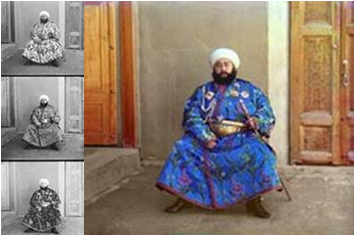
\includegraphics[width=0.65\linewidth]{example-Prokudin-Gorskii.png}
\caption{\label{fig:align} Example image from the Prokudin-Gorskii collection. On the left are the three images captured individually. On the right is a reconstructed color photograph. Note the colors are in B, G, R order from the top to bottom (and not R, G, B)!}
\end{figure}

Your goal is to take photographs of each plate and generate a color image by aligning them (Figure~\ref{fig:align}). The easiest way to align the plates is to exhaustively search over a window of possible displacements, say [-15,15] pixels, score each one using some image matching metric, and take the displacement with the best score. There is a number of possible metrics that one could use to score how well the images match. The simplest one is just the L2 norm also known as the Sum of Squared Differences (SSD) distance which is simply \cmd{sum(sum((image1-image2)$.^\wedge$2))} where the sum is taken over the pixel values. Another is normalized cross-correlation (NCC), which is simply a dot product between two normalized vectors: \cmd{(image1./||image1||} and \cmd{image2./||image2||)}. Note that in the case of the Emir of Bukhara (Figure 1), the images to be matched do not actually have the same brightness values (they are different color channels), so the distance between them will not be zero even after alignment.

\subsection{Code}
Before you get started make sure you know the basics of programming in MATLAB/Python. Then download the \cmd{p1.zip} and \cmd{p1.pdf} from the moodle. Move them to your homework directory and extract the files (e.g. by typing \cmd{unzip p1.zip}). The codes are available in the directory \cmd{p1/code}.
The latex sources are also available as \cmd{p1/latex}.  

Before you start aligning the Prokudin-Gorskii images (in $\cmd{data/prokudin-gorskii}$), you will test your code on synthetic images which have been randomly shifted. Your code should correctly discover the inverse of the shift. Take a look at this code and see how the test examples are generated. Run \cmd{evalToyAlignment} on the Matlab command prompt inside the code directory. This should produce the following output. Note the actual 'gt shift' might be different since it is randomly generated.
\begin{verbatim}
    Evaluating alignment ..
    1 balloon.jpeg
	   gt shift: ( 1,11) ( 4, 5)
	 pred shift: ( 0, 0) ( 0, 0)
    2 cat.jpg
	   gt shift: (-5, 5) (-6,-2)
	 pred shift: ( 0, 0) ( 0, 0)
     ...
\end{verbatim}
    
The code loads a set of images, randomly shifts the color channels and provides them as input to \cmd{alignChannels}. 
\textbf{Your goal is to implement this function.}
A correct implementation should obtain the shifts that are the negation of the ground-truth shifts producing the following output:

\begin{verbatim}
    Evaluating alignment ..
    1 balloon.jpeg
	   gt shift: ( 13, 11)  ( 4, 5)
	 pred shift: (-13,-11)  (-4,-5)
    2 cat.jpg
	   gt shift: (-5, 5) (-6,-2)
	 pred shift: ( 5,-5) ( 6, 2)
     ...
\end{verbatim}
    
Once you are done with that, run \cmd{evalProkudinAlignment}. This will call your function to align images from the Prokudin-Gorskii collection stored in \cmd{data/prokudin-gorskii} directory. The output is saved to the \cmd{outDir}.


\subsection{What to submit?}
To get full credit for this part you have to 
\begin{itemize}
\item Include your implementation of \cmd{alignChannels}
\item Verify that the \cmd{evalAlignment} correctly recovers the color image and shifts for the toy example and include the output results.
\item Show the aligned color images from the output of \cmd{alignProkudin} and the computed shift vectors for each image.
\end{itemize}

\subsection{Some tips}
\begin{itemize}
\item Look at functions \cmd{circshift()} and \cmd{padarray()} to deal with shifting images in MATLAB.
In Python, look for \cmd{np.roll} and \cmd{np.pad}.

\item The ``verbatim" package provides ways to include pasted code, or code from a file, in its raw format. For example the code in a file \cmd{alignChannels} can be included in Latex by typing: 
\begin{verbatim}
\verbatiminput{../solution/alignChannels.m}}.
\end{verbatim}

\item Shifting images can cause ugly boundary artifacts. You might find it useful to crop the image after the alignment.
\end{itemize}



\newpage

\section{Photometric stereo [50 points]}


In this part you will implement a basic shape-from-shading algorithm as described in Lecture 5. This is also described in the ``shape from shading" section (Sec 2.2) in Forsyth and Ponce book (\href{http://www.sci.utah.edu/~gerig/CS6320-S2012/Materials/Forsyth-Ponce-SfS.pdf}{pdf link} for this section). The input to the algorithm is a set of photographs taken with known lighting directions and the output of the algorithm is the albedo (paint), normal directions, and the height map (Figure~\ref{fig:photometric-stereo}).


If you haven't done so already, download the \cmd{p1.zip} and \cmd{p1.pdf} files from Moodle. The \cmd{data/ photometricStereo} directory consists of 64 images each of four subjects from the Yale Face database. The light source directions are encoded in the file names. 


\begin{figure}[h]
\centering
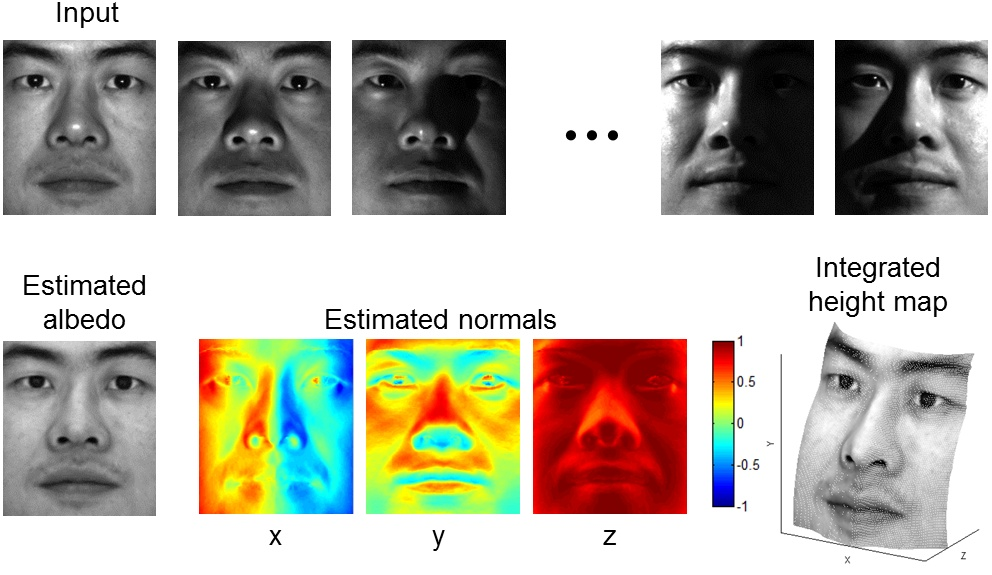
\includegraphics[width=0.85\linewidth]{shape_from_shading.jpg} \\
\caption{\label{fig:photometric-stereo} Top row: Input images. Bottom row: Estimated albedo, normals, and depth map}
\end{figure}


Below is an outline of the steps you need to implement the functions. The entry code for this part is \cmd{evalPhotometricStereo}. You will add code to files \cmd{prepareData}, \cmd{photometricStereo} and \cmd{getSurface} as described below. The remaining files are for processing the input data and displaying the output.

\begin{enumerate}

\item \textbf{Read images and light sources.} For each subject (sub-directory in the \cmd{data} folder), read in the images and light source directions. This is accomplished by the function \cmd{loadFaceImages} (which, in turn, calls \cmd{getpgmraw} to read the PGM files). The function \cmd{loadFaceImages()} returns the images for the 64 light source directions, an ambient image (i.e., image taken with all the light sources turned off), and the light directions for each image.

\item \textbf{[5 points] Preprocess the data.} We need the images under the illumination of only the point light source. Fortunately, due to linearity of light we can do this by subtracting the ambient image from all the images. Also, set any negative values to zero and rescale the resulting intensities to between 0 and 1. Implement this in the \cmd{prepareData} file.


\item \textbf{[20 points] Estimate the albedo and  normals.} Implement the function  \cmd{photometricStereo}, which takes as input the stack of images and the light source directions, and returns an albedo image and normal directions. The normal directions can be encoded as a three dimensional array of size $h \times w \times 3$ where the third dimension corresponds to the x-, y-, and z-components of the normal of each pixel. 


To solve for the albedo and the normals, you will need to set up a linear system of equations as described in Lecture 2. To get the least-squares solution of a linear system, use MATLAB's backslash operator. That is, the solution to \cmd{Ax = b} is given by \cmd{x = A\textbackslash b}.
In Python, you can use \cmd{scipy.linalg.lstsq}. For this homework some useful MATLAB functions are \cmd{reshape}, \cmd{cat} and \cmd{bsxfun}.
You may also need to use element-wise operations. For example, for two equal-sized matrices $\mathbf{X}$ and $\mathbf{Y}$, the operation $\mathbf{X}$.* $\mathbf{Y}$ multiplies corresponding elements, and $\mathbf{X}.^\wedge 2$ squares every element.
In Python, element-wise operations correspond to the standard operators and matrix multiplication is done
through the \cmd{np.array} member function \cmd{dot}.

\item \textbf{[20 points] Compute the surface height map by integration.} The method is shown in Lecture 2, except that instead of continuous integration of the partial derivatives over a path, you will simply be summing their discrete values. Your code implementing the integration should go in the \cmd{getSurface} file. As stated in the slide, to get the best results, you should compute integrals over multiple paths and average the results. You should implement the following variants of integration: 
\begin{itemize}
\item Integrating first the rows, then the columns. That is, your path first goes along the same row as the pixel along the top, and then goes vertically down to the pixel. It is possible to implement this without nested loops using the \cmd{cumsum()} function.
\item Integrating first along the columns, then the rows.
\item Average of the first two options.
\item Average of multiple random paths. For this, it is fine to use nested loops. You should determine the number of paths experimentally.
\end{itemize}

\item Display the results using \cmd{displayOutput} and \cmd{plotSurfaceNormals} functions.

\end{enumerate}

\textbf{Hint:} You can start by setting the \cmd{subjectName='debug'} which creates images from a toy scene with known geometry and albedo. You can debug your code against this before you try the faces.

\subsection{What to submit}
To get full credit for this part you have to
\begin{itemize}
\item Include your implementation of \cmd{prepareData}, \cmd{photmetricStereo}, and \cmd{getSurface}. Also, include the visualization of albedo image, estimated surface normals, and recovered surface of four subjects. It is sufficient to simply show the output of your best method. For the 3D screenshots, be sure to choose a viewpoint that makes the structure as clear as possible (and/or feel free to include screenshots from multiple viewpoints)
\item \textbf{[5 points]} Discuss the differences between the different integration methods you have implemented. Specifically, you should choose one subject, display the outputs for all of a-d (be sure to choose viewpoints that make the differences especially visible), and discuss which method produces the best results and why. Also, discuss how the Yale Face data violate the assumptions of the shape-from-shading method covered in the slides.
\end{itemize}

\section{Report Writing and Presentation [10 points]}

Please follow the guidelines for writing a good report.
Graders will penalize reports that are poorly written or fail to present the results in a reasonable manner.


\section{Extensions for extra credit}
You can get up to 10\% extra credit for this homework by substantially improving the baseline algorithm. Some of these may even be research questions that can be explored in the final project. 
On this assignment, there are not too many opportunities for "easy" extra credit. This said, here are some ideas for exploration:
\begin{itemize}
\item Generate synthetic input data using a 3D model and a graphics renderer and run your method on this data. Do you get better results than on the face data? How close do you get to the ground truth (i.e., the true surface shape and albedo)?
\item Investigate more advanced methods for shape from shading or surface reconstruction from normal fields.
\item Try to detect and/or correct misalignment problems in the initial images and see if you can improve the solution.
\item Using your initial solution, try to detect areas of the original images that do not meet the assumptions of the method (shadows, specularities, etc.). Then try to recompute the solution without that data and see if you can improve the quality of the solution.
\end{itemize}
If you complete any work for extra credit, be sure to clearly mark that work in your report, explain it and include the code.



\end{document}


